%% Submissions for peer-review must enable line-numbering 
%% using the lineno option in the \documentclass command.
%%
%% Preprints and camera-ready submissions do not need 
%% line numbers, and should have this option removed.
%%
%% Please note that the line numbering option requires
%% version 1.1 or newer of the wlpeerj.cls file.


\documentclass[fleqn,10pt,lineno]{wlpeerj} % for journal submissions
%\documentclass[fleqn,10pt]{wlpeerj} % for preprint submissions


%\newcommand{\rr}{${\mathcal{R}}$}
\usepackage{amssymb}
\usepackage{amsmath}
\usepackage{upgreek}
\usepackage[]{fontenc}
\usepackage{color}
\usepackage{bm}
\usepackage[english]{babel}
\usepackage{graphicx}
\usepackage{tikz}
\usetikzlibrary{positioning}
\usepackage{ifthen}
\usepackage{xstring}
\usepackage{afterpage}
%\usepackage[hidelinks]{hyperref}
\usepackage[colorlinks=true, allcolors=blue, pdfborder={0 0 0}]{hyperref}


% ==============

% ========================================================================================
% ========================================================================================
\usepackage[utf8]{inputenc}
\DeclareFixedFont{\ttb}{T1}{txtt}{bx}{n}{9} % for bold
\DeclareFixedFont{\ttm}{T1}{txtt}{m}{n}{9}  % for normal
% Defining colors
\usepackage{color}
\definecolor{deepblue}{rgb}{0,0,0.5}
\definecolor{deepred}{rgb}{0.6,0,0}
\definecolor{deepgreen}{rgb}{0,0.5,0}
\usepackage{listings}
\usepackage{textcomp} 
\usepackage[T1]{fontenc}
% for upquotes
\newcommand\pythonstyle{\lstset{
  language=Python,
  backgroundcolor=\color{white}, %%%%%%%
  % basicstyle=\ttm,
  basicstyle=\footnotesize,
  numbers=right,
  stepnumber=1,
  otherkeywords={self},            
  keywordstyle=\ttb\color{deepblue},
  emph={MyClass,__init__},          
  emphstyle=\ttb\color{deepred},    
  stringstyle=\color{deepgreen},
  commentstyle=\color{red},  %%%%%%%%
  frame=tb,                         
  showstringspaces=false,
  upquote=true,
  %obeytabs=true,
  tabsize=2
}}

% Python environment
\lstnewenvironment{python}[1][]
{
\pythonstyle
\lstset{#1}
}
{}

% Python for external files
\newcommand\pythonexternal[2][]{{
\pythonstyle
\lstinputlisting[#1]{#2}}}

% Python for inline
\newcommand\pythoninline[1]{{\pythonstyle\lstinline!#1!}}

\def\ContinueLineNumber{\lstset{firstnumber=last}}
% ========================================================================================
% ========================================================================================

\newcommand{\floor}[1]{\left \lfloor #1 \right \rfloor}
\newcommand{\round}[1]{\left \lfloor #1 \right \rceil }
\newcommand{\ceil}[1]{\left \lceil #1 \right \rceil }
\newcommand{\Fig}[1]{Fig.~\ref{#1}}
%\newcommand{\Fig}[1]{Figure~\ref{#1}}
\newcommand{\Figs}[1]{Figs.~\ref{#1}}
%\newcommand{\Figs}[1]{Figures~\ref{#1}}
\newcommand{\Sec}[1]{Section~\ref{#1}}
\newcommand{\Secs}[1]{Sections~\ref{#1}}
\newcommand{\Chap}[1]{Chapter~\ref{#1}}
\newcommand{\Chaps}[1]{Chapters~\ref{#1}}
\newcommand{\Tab}[1]{Table~\ref{#1}}
\newcommand{\Tabs}[1]{Tables~\ref{#1}}
\newcommand{\Eqn}[1]{Eqn.~\ref{#1}}
\newcommand{\Eqns}[1]{Eqns.~\ref{#1}}
\newcommand{\InEqn}[1]{Inequality~(\ref{#1})}
\newcommand{\InEqns}[1]{Inequalities~(\ref{#1})}
\newcommand{\Center}[1]{\textcolor{white}{.}\hfill#1\hfill\textcolor{white}{.}}
\newcommand{\ang}{$\textrm\AA$}
\newcommand{\new}[1]{#1}
\newcommand{\New}[1]{#1}
\newcommand{\n}[1]{#1}
\newcommand{\we}{I~}

\usepackage{xspace}

\newcommand{\gname}{BackMap}
\newcommand{\pname}{\textsc{\gname}\xspace}
\newcommand{\code}[1]{\texttt{#1}\xspace}

\usepackage[cal=cm,scrscaled=1.05]{mathalfa} % This is for \mathcal{}, particularly \mathcal{R}
\DeclareMathAlphabet\mathbfcal{OMS}{cmsy}{b}{n} % for boldface mathcal: \mathbfcal{}
\newcommand{\rr}{$\mathcal{R}$\xspace}

\def\kt{k_{\rm B}T}

\def\beq{\begin{equation}}
\def\eeq{\end{equation}}
\def\bea{\begin{eqnarray}}
\def\eea{\end{eqnarray}}

\def\cal#1{\mathcal{#1}}
\def\eqq#1{Eq.~(\ref{#1})}
\def\eq#1{(\ref{#1})}
\def\av#1{\langle #1 \rangle}

\def\f#1{Fig.~\ref{#1}}
\def\ff#1{Figs.~\ref{#1}}

\def\s#1{Section~\ref{#1}}

\def\c#1{~\cite{#1}}


%\newcommand{\c}[1]{\citep{#1}}

\newcommand{\figdir}{../figures}

\title{The Backmap Python Module: How a Simpler Ramachandran Number Can Simplify the Life of a Protein Simulator}


\author[*]{Ranjan V. Mannige}
%\author[1,2,*]{Ranjan V. Mannige}
%\affil[1]{~KPMG, Atlanta, CA 30309, U.S.A.}
%\affil[2]{~Multiscale Institute, Atlanta, CA 30309, U.S.A.}
\affil[*]{~ranjanmannige@gmail.com}

%\keywords{Ramachandran number, Multi-angle Picture, MAP, Protein structure}

\begin{abstract}
Protein backbones display complicated structures that often undergo numerous types of structural transformations. Due to the large number of structural degrees of freedom available to a backbone, it is often difficult to assess exactly where and how regions of a protein structure undergo structural transformation. This large structural phase makes it hard to survey new structural data, such as molecular dynamics trajectories or NMR-derived structural ensembles. This report discusses the Ramachandran number \rr as a residue-level structural metric that could simply the life of anyone contending with large numbers of structural data associated with protein backbones. In particular, this report 1) discusses a much simpler closed form of \rr that makes it more easy to calculate, 2) shows how \rr dramatically reduces the dimensionality of the protein backbone, thereby making it ideal for simultaneously interrogating large number of protein structures. In short, \rr is a simple and succinct descriptor of protein backbones and their dynamics.
\end{abstract}

\begin{document}

\flushbottom
\maketitle
\thispagestyle{empty}

\section*{Introduction}

Proteins are a class of biomolecules unparalleled in their functionality \citep{Berg2006}. A natural protein may be thought of as a linear chain of amino acids, each normally sourced from a repertoire of 20 naturally occurring amino acids. 
%Its exact sequence of amino acids (its primary sequence) dictates much about the final conformation fo a protein. E.g., a protein of a specific sequence may repeatedly fold into (or assume) a certain three-dimensional conformation \citep{Berg2006}. 
Proteins are important partially because of the structures that they access: the conformations (conformational ensemble) that a protein assumes determines the functions available to that protein. However, all proteins are dynamic: even stable proteins undergo long-range motions in its equilibrium state; i.e., they have substantial diversity in their conformational ensemble \citep{Mannige2014b}. Additionally, a number of proteins undergo conformational transitions, without which they may not properly function. Finally, some proteins -- intrinsically disordered proteins -- display massive disorder whose conformations dramatically change over time \citep{Uversky2003, Fink2005, Midic2009, Espinoza-Fonseca2009, Uversky2010, Tompa2011, Sibille2012, Kosol2013, Dunker2013, Geist2013, Baruah2015}, and whose characteristic structures are still not well-understood \citep{Beck2008}.

\begin{figure}[b!]
\centering
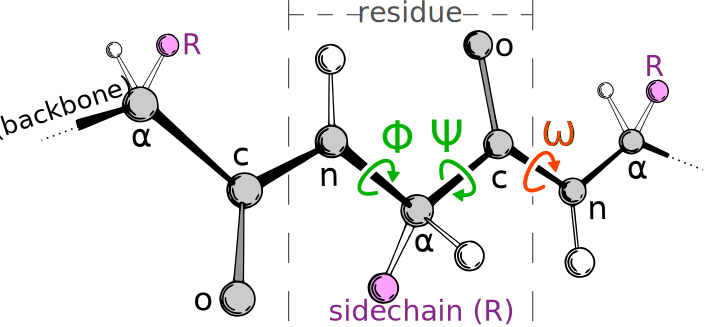
\includegraphics[width=0.4\linewidth]{figures/peptide_small.pdf}
\caption{\textbf{Backbone conformational degrees of freedom} dominantly depend on the dihedral angles $\phi$ and $\psi$ (green), and to a smaller degree depend on the third dihedral angle ($\omega$; red) as well as bond lengths and angles (unmarked). \label{fig:intro}} 
\end{figure}


Large-scale changes in a protein occur due to changes in protein backbone conformations. %\footnote{Sidechain conformational changes alone, while correlated in space and time -- see \cite{DuBay2011} -- can not alone contribute to the change in a protein fold/conformation.}. 
\Fig{fig:intro} is a cartoon representation of a peptide/protein backbone, with the backbone bonds themselves represented by darkly shaded bonds. \cite{Ramachandran1963} had recognized that the backbone conformational degrees of freedom available to an amino acid (residue) $i$ is almost completely described by only two dihedral angles: $\phi_i$ and $\psi_i$ (\Fig{fig:intro}, green arrows). %A third dihedral angle, $\omega_i$, is primarily planar at $180^\circ$; \cite{Pauling1951a,Pauling1951}]\footnote{See \Fig{fig:intro}a. For any amino acid $i$, $\phi_i$, $\psi_i$ and $\omega_i$ respectively involve the four atoms $\{\mathrm{C}_\mathrm{-1}, \mathrm{N}, \mathrm{C}\upalpha, \mathrm{C}\}$, $\{\mathrm{N}, \mathrm{C}\upalpha, \mathrm{C}, \mathrm{N}_\mathrm{+1}\}$, and  $\{\mathrm{C}\upalpha_\mathrm{-1}, \mathrm{C_{-1}}, \mathrm{N},\mathrm{C}\upalpha\}$.The central bond involving $\omega_i$ describes the amide bond connecting residues $(i-1)$ and $i$. An alternative $\omega_i$ involves the connection between residues $i$ and $(i+1)$, where the four relevant atoms are $\{\mathrm{C}\upalpha, \mathrm{C}, \mathrm{N_{+1}},\mathrm{C}\upalpha_{+1}\}$.}. 
Today, protein structures described in context of the two-dimensional $(\phi,\psi)$-space are called Ramachandran plots.

The Ramachandran plot is recognized as a powerful tool for two reasons: 1) it serves as a map for structural `correctness' \citep{Laskowski1993,Hooft1997,Laskowski2003}, since many regions within the Ramachandran plot space are energetically not permitted \citep{Momen2017}; and 2) it provides a qualitative snapshot of the structure of a protein \citep{Berg2006,Alberts2002,Subramanian2001}. For example, particular regions within the Ramachandran plot indicate the presence of particular secondary locally-ordered structures such as the $\upalpha$-helix and $\upbeta$-sheet (see \Fig{fig:ramaintro}a).

While the Ramachandran plot has been useful as a measure of protein backbone conformation, it is not popularly used to assess structural dynamism and transitions (unless specific knowledge exists about whether a particular residue is believed to undergo a particular structural transition). This is because of the two-dimensionality of the plot: describing the behavior of every residue involves tracking its position in two-dimensional ($\phi$,$\psi$) space. For example, a naive description of positions of a peptide in a Ramachandran plot (\Fig{fig:ramaintro}b) needs more annotations for a per-residue analysis of the peptide backbone's structure. Given enough residues, it would be impractical to track the position of each residue within a plot. This is compounded with time, as each point in (b) becomes a curve (c), further confounding the situation. The possibility of picking out previously unseen conformational transitions and dynamism becomes a logistical impracticality. As indicated above, this impracticality arises primarily from the fact that the Ramachandran plot is a two-dimensional map.

\begin{figure*}[t!]
\centering
\includegraphics[width=1.0\linewidth]{automated_figures/fig_rama_intro.pdf}
\caption{While the Ramachandran plot is useful for getting a {\it qualitative} sense of peptide backbone structure (a, c), it is not a convenient representation for exploring peptide backbone dynamics (c).\label{fig:ramaintro}} 
\end{figure*}

Consequently, there has been no single compact descriptor of protein structure. This impedes that na{\"i}ve or hypothesis-free exploration of new trajectories/ensembles. %\footnote{Of course, if prior knowledge (or hypothesis) existed that a structural transition occurred along a specific reaction coordinate -- say with the change in a particular atom-atom distance and or a particular dihedral angle -- then na{\"i}ve exploration would not be required. However, even in these situations, \pname would be important to provide structural fingerprints (see \Fig{fig:metrics}).}. 
For example, tracking changes in protein trajectory is either overly detailed or overly holistic: an example of an overly detailed study is the tracking on exactly one or a few atoms over time (this already poses a problem, since we would need to know exactly which atoms are expected to partake in a transition); an example of a holistic metric is the radius of gyration (this also poses a problem, since we will never know which residues contribute to a change in radius of gyration without additional interoogation). % While these metrics are heavily used by the molecular dynamics community, the change in these metrics over time only provides a general sense that something in the structure is changing. These metrics, however, can not provide any more residue-level details than that. 
With protein dynamics undergoing a new rennissance -- especially due to intrinsically disordered proteins and allostery -- having hypothesis-agnostic yet detailed (residue-level) metrics of protein structure has become even more relevant. 
%The Ramachandran number provides just such a middle ground by being compact enough to simply describe residue-level structural information Below, we will attempt to show that the Ramachandran number ($\mathcal{R}$), and the multi-angle picture, described below, is much more informational than prior ``na{\"i}ve metrics''.

\begin{figure}[t!]
\centering
\includegraphics[width=0.6\linewidth]{automated_figures/fig_ss_2d_1d.pdf}
\caption{The distribution of dominant regular secondary sctuctures are shown in $[\phi,\psi]$-space (a) and in $\mathcal{R}$-space (b). Both Ramachandran plots (a) and Ramachandran `lines' (b) show equivalent resolution of secondary structure , allowing for a more compact representation of Ramachandran plots \cite{Mannige2016}.\label{fig:ramasecondary}} 
\end{figure}

It has recently been shown that the two Ramachandran backbone parameters ($\phi$,$\psi$) may be conveniently combined into a single number -- the Ramachandran \textit{number} [$\mathcal{R}(\phi,\psi)$ or simply $\mathcal{R}$] -- with little loss of information \citep{Mannige2016}. 
In a previous report, detailed discussions were provided regarding the reasons behind and derivation of $\mathcal{R}$ \citep{Mannige2016}. This report provides a simpler version of the equation previously published \citep{Mannige2016}, and further discusses how $\mathcal{R}$ may be used to provide information about protein ensembles and trajectories. 
%We call these pictograms ``MAPs'' (or simply ``maps''), an acronym for Multi-Angle Pictures. 
Finally, we introduce a software package -- \pname -- that can be used by to produce MAPs that describe the behavior of a protein backbone within user-inputted conformations, structural ensembles and trajectories. This package is presently available on GitHub (\url{https://github.com/ranjanmannige/\gname}).

\section*{Introducing the \textit{simplified} Ramachandran number ($\mathcal{R}$)}

%Before expanding on the utility of the Ramachandran number, this section will present the Ramachandran number, after which a much simpler (and more accurate) version of the Ramachandran number will be described.
The Ramachandran number is both an idea and an equation. Conceptually, the Ramachandran number ($\mathcal{R}$) is any closed form that collapses the dihedral angles $\phi$ and $\psi$ into one structurally meaningful number \citep{Mannige2016}. \cite{Mannige2016} presented a version of the Ramachandran number that was complicated in closed form, threby reducing its utility. Here, a much more simplified version of the Ramachandran number is introduced. Section~\ref{sec:simplifyR} shows how this simplified form was derived from the original closed form (\Eqns{rama} and \ref{ramachandran_raw}).

%Assuming the bounds $\phi,\psi \in [-180^\circ,180^\circ)$, and the range $\lambda$ equals $360^\circ$, the {\it simplified} 

Given arbitrary limits of $\phi \in [\phi_{\rm min},\phi_{\rm max})$ and $\psi \in [\psi_{\rm min},\psi_{\rm max})$, where the minimum and maximum values differ by $360^\circ$, the most general and accurate equation for the Ramachandran number is
\begin{equation}
{\mathcal{R}}(\phi,\psi) \equiv  \frac{\phi+\psi-(\phi_{\rm min}+\psi_{\rm min})}{(\phi_{\rm max}+\psi_{\rm max})-(\phi_{\rm min}+\psi_{\rm min})}.
\label{ramaGeneral}
\end{equation}

For consistency, we maintain throughout this paper that $\phi_{\rm min} = \psi_{\rm min} = -180^\circ$ or $-\uppi$ radians, which makes 
\begin{equation}
\mathcal{R}(\phi,\psi) = \frac{\phi+\psi+2\uppi}{4\uppi}.\label{eqn:rama}
\end{equation}

%Section~\ref{sec:simplifyR} delineates how this equation can be derived from the original closed form described in \cite{Mannige2016}.

As evident in \Fig{fig:ramasecondary}, the distributions within the Ramachandran plot are faithfully reflected in corresponding distributions within Ramachandran number space. This paper  shows how the Ramachandran number is both compact enough and informative enough to generate immediately useful graphs (map) of a dynamic protein backbone.

\section*{Reason to use the Ramachandran Number}

\subsection*{Ramachandran numbers are more compact than one might realize}

\begin{figure}[t!]
\centering
\includegraphics[width=0.65\linewidth]{figures/fig2_metrics.pdf}
\caption{\textbf{Two types of $\mathcal{R}$-codes.} Digesting protein structures (a) using $\mathcal{R}$ numbers either as histograms (b) or per-residue codes (c) allow for compact representations of salient structural features. For example, a single glance at the histograms indicate that protein 1mba is likely all $\upalpha$-helical, while 2acy is likely a mix of $\upalpha$-helices and $\upbeta$-sheets. Additionally, residue-specific codes (c) not only indicate secondary structure content, but also exact seconday structure stretches (compare to d), which gives a more complete picture of how the protein is linearly arranged. \label{fig:simple_stacks}} 
\end{figure}

An important aspect of the Ramachandran number ($\mathcal{R}$) lies in its compactness compared to the traditional Ramachandran pair ($\phi,\psi$). Say we have an $N$-residue peptide. Then, switching from ($\phi,\psi$) to $\mathcal{R}$ \textit{appears} to only reduce the number of variables from $2N$ to $N$, and hense by half. However, ($\phi,\psi$) values are {\it coupled}, i.e., for any $N$-length peptide, any ordering of $[\phi_1,\phi_2,\ldots,\phi_N,\psi_1,\psi_2,\ldots,\psi_N]$ can not describe the structure, it is only \textit{pairs} -- $[(\phi_1,\psi_1),(\phi_2,\psi_2),\ldots,(\phi_N,\psi_N)]$ -- that can. Therefore, we must think of switching from ($\phi,\psi$)-space to $\mathcal{R}$-space as a switch in structure space per residue from $N$ two-tuples $(\phi_i,\psi_i)$ that reside in $\phi\times\psi$ space to $N$ single-dimensional numbers ($\mathcal{R}_i$).

The value of this conversion is that the structure of a protein can be described in various one-dimensional arrays (per-structure ``Ramachandran codes'' or ``$\mathcal{R}$-codes''), which, when arranged vertically/columnarly, consititue easy to digest codes. See, e.g., \Fig{fig:simple_stacks}. 

\begin{figure}[t!]
\centering
\includegraphics[width=0.65\linewidth]{figures/nano_r_demo.pdf}
\caption{\textbf{Stacked $\mathcal{R}$-codes provide useful information at a glance.} \label{fig:complex_stacks}} 
\end{figure}

\subsection*{Ramachandran codes are stackable}

In addition to assuming a small form factor, $\mathcal{R}$-codes may then be \textit{stacked} side-by-side for visual and computational analysis. There lies its true power.

For example, the one-$\mathcal{R}$-to-one-residue mapping means that the entire residue-by-residue structure of a protein can be shown using a string of $\mathcal{R}_i$s (which would show regions of secondary structure and disorder, for starters). Additionally, an entire protein's backbone makeup can be shown as a histogram in $\mathcal{R}$-space (which may reveal a protein's topology). The power of this format lies not only in the capacity to distill complex structure into compact spaces, but in its capacity to display {\it many} complex structures in this format, side-by-side (stacking).

Peptoid nanosheets \citep{Mannige2015} will be used here as an example of how multiple structures, in the form of \rr-codes, may be stacked to provide immediately useful pictograms. Peptoid nanosheets are a recently discovered peptide-mimic that were shown to display a novel secondary structure \citep{Mannige2015}. In particular, each peptoid within the nanosheet displays backbone conformations that alternate in chirality, causing the backbone to look like a meandering snake that nonetheless maintains an overall linear direction. This secondary structure was discovered by first setting up a nanosheet where all peptoid backbones are restrained in the extended format (\Fig{fig:complex_stacks}a, left), after which the restraints were energetically softened (a, middle) and completely reseased (a, right). As evident in \Fig{fig:complex_stacks}b and \Fig{fig:complex_stacks}c, the two types of \rr-code stacks display salient information at first glance: 1) \Fig{fig:complex_stacks}b shows that the extended backbone first undergoes some rearrangement with softer restraints, and then becomes much more binary in arrangement as we look down the backbone (excepting the low-order region in the middle, unshown in \Fig{fig:complex_stacks}a); and 2) \Fig{fig:complex_stacks}c shows that lifting restraints on the backbone causes a dramatic change in backbone topology, namely a birth of a bimodal distribution evident in the two parallel bands.

By utilizing \rr, maps such as those in \Fig{fig:complex_stacks} provide information about every $\phi$ and $\psi$ within the backbone. As such, these maps are dubbed MAPs, for Multi Angle Pictures. A Python package called \pname created \Fig{fig:complex_stacks}a and b, which is provided as a GitHub repository at \url{https://github.com/ranjanmannige/\gname}. \pname takes in a PDB structure file containing a single structure, or multiple structures separated by the code `MODEL'.

\subsection*{Other uses for \rr: picking out subtle differences from high volume of data}

This section expands on the notion that \rr-numbers -- due to their compactness/stackability -- can be used to pick out backbone structural trends that would be hard to decipher using any other metric. For example, it is well known that prolines (P) display unusual backbone behavior: in particular, proline backbones occupy structures that are close to but distinct from $\upalpha$-helical regions. Due to the two-dimensionality of Ramachandran plots (\Fig{fig:peraa}a), such distinctions are hard to visually pick out from Ramachandran plots. However, stacking per-amino-acid \rr-codes side by side make such differences patent (\Fig{fig:peraa}b; see arrow).

\begin{figure*}
\centering
\includegraphics[width=0.97\linewidth]{automated_figures/fig_ramachandran_plots_vs_numbers.pdf}
\caption{\textbf{Ramachandran lines are stackable -- Part I.}  
Panel (a) shows the per-amino acid backbone behavior of an average protein found in the protein databank (PDB). While these plots are useful, it is difficult to compare such plots. For example, it is hard to pick out the change in the $\upalpha$-helial region of the proline plot (P). However, when we convert Ramachandran plots to Ramachanran \textit{lines} [by converting $(\phi_i,\psi_i)\to\mathcal{R}_i$], we are able to conveniently ``stack'' Ramachandran lines calculated for each residue. Then, even visually, it is obvious that proline does not occupy the canonical $\upalpha$-helix region, which is not evident to an untrained eye in (a).\label{fig:peraa}}
~\vfill~
\includegraphics[width=0.97\linewidth]{automated_figures/fig_ramachandran_numbers_are_useful1.pdf}
\caption{\textbf{Ramachandran lines are stackable -- Part II.} Similar to \Fig{fig:peraa}b, Panel (a) represents the behavior of an amino acid `Y' situated {\it before} a leucine (assuming that we are reading a sequence from the N terminal to the C terminal). Panel (b) similarly represents the behavior of specific amino acids situated before a proline. While residues preceeding a leucine behave similarly to their average behavior (\Fig{fig:peraa}a), most residues preceeding prolines appear to be enriched in structures that change `direction' or backbone chirality (\rr$>0.5$). Panel (c) shows the behavior of individual amino acids when situated before each of the 20 amino acids. This graph shows a major benefit of side-by-side Ramachandran line ``stacking'': general trends become much more obvious. For example, it is evident that glycines and prolines dramatically modify the structure of an amino acid preceeding it (compared to average behavior of amino acids in \Fig{fig:peraa}b). This trend is not as strong when considering amino acids that {\it follow} glycines or prolines (c). Such trends, while previously discovered [e.g., \cite{Gunasekaran1998,Ho2005}], would not be accessible when na{\"i}vely considering Ramachandran plots because one would require 400 ($20\times 20$) distinct Ramachandran plots to compare. %Panel (d) facetiously represents 800 tiny Ramachandran plots, emphasizing how hard it would be to make such comparisons using Ramachandran plots.
\label{fig:motifs}}
\end{figure*}

It is also known that amino acids preceeding prolines display unusual shift in chirality. For example, \Fig{fig:motifs} shows that amino acids appearing before prolines and glycines behave much more differently than they would otherwise. While these results have been discussed previously \citep{Gunasekaran1998,Ho2005}, they were reported more than 30 years after the first structures were published; they would have been relatively easy to find if \rr-codes were to be used regularly. 

The relationships in \Figs{fig:peraa} and \ref{fig:motifs} show how subtle changes in structure can be easily picked out when structures are stacked side-by-side in the form of $\mathcal{R}$-codes. Such subtle changes are often witnessed when protein backbones transition from one state to another.

\section*{Using the \pname Python Module}

\subsection*{Installation}
\pname may either be downloaded from the github repository, or installed directly by running the following line in the command prompt (assuming that pip exists): \code{> pip install backmap}

\subsection*{First smple test}
The simplest test would be to generate Ramachandran numbers from $(\phi,\psi)$ pairs:
\begin{python}
# Import module
import backmap 
# Convert (phi, psi) to R
print backmap.R(phi=0,phi=0) # Expected output: 0.5
print backmap.R( -180, -180) # Expected output: 0.0
print backmap.R(  180,  180) # Expected output: 1.0 (equivalent in meaning to 0)
\end{python}

\subsection*{Basic usage for creating Multi-Angle Pictures (MAPs)}
As seen above, the generation of Ramachandran numbers from $(\phi,\psi)$ pairs is simple. However, greating MAPs -- Multi-Angle Pictures of protein backbones -- requires a few more steps (present as a test in the downloadable module):
\begin{enumerate}
\item {\bf Select and read a protein PDB structure}\\
Each trajectory frame must be a set of legitimate protein databank "ATOM" records separated by "MODEL" keywords.
\begin{python}[firstnumber=1]
import backmap 
pdbfn = './pdbs/nanosheet_birth_U7.pdb' # Set pdb name 
data = backmap.read_pdb(pdbfn) # READ PDB in the form of a matrix with columns
\end{python}
Here, `\code{data}' is a 2d array with four columns [`\code{model}', `\code{chain}', `\code{resid}',`\code{R}']. 
The first row of `\code{data}' is the header (i.e., the name of the column, e.g., `\code{model}'), 
with values that follow.
\item {\bf Select color scheme (color map)}\\
In addition to custom colormaps listed in the next section, one can also use standardly available at 
\href{http://matplotlib.org/examples/color/colormaps_reference.htm}{matplotlib.org} (e.g., `\code{Reds}' or `\code{Reds\_r}').
\ContinueLineNumber
\begin{python}
# setting the name of the colormap
cmap = "SecondaryStructure"
\end{python}
\item {\bf Draw per-chain MAPs}
\ContinueLineNumber
\begin{python}
# Grouping by chain
grouped_data = backmap.group_by(data,group_by='chain',
                            columns_to_return=['model','resid','R'])
for chain in grouped_data.keys(): # Going through each chain
	# Getting the X,Y,Z values for each entry
	models, residues, Rs = grouped_data[chain]
	# Finally, creating (but not showing) the graph 
	backmap.draw_xyz(X = models  ,      Y = residues  ,     Z = Rs
	           ,xlabel ='Frame #', ylabel ="Residue #",zlabel ='$\mathcal{R}$'
	             ,cmap = cmap    ,  title = "Chain: '"+chain+"'"
	             ,vmin=0,vmax=1)
	# Now, we display the graph:
	plt.show() # ... one can also use plt.savefig() to save to file
\end{python}
As one would expect, this is the business end of the code. By changing how one assigns values to `X' and `Y', 
one can easily construct and draw other types of graphs such as time-resolved histograms, 
root mean squared fluctuations, root mean squared deviation, etc. 
Running the module as a standalone script would produce all these graphs automatically.
`\code{plt.show()}' would result in the following image being rendered:\\
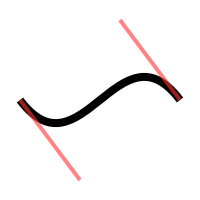
\includegraphics[width=0.5\linewidth]{automated_figures/example.pdf}
\end{enumerate}

\subsection*{Creating custom graphs}
Other types of grpahs can be easily created by modifying part three of the code above. 
For example, the following code creates histograms of R, one for each model (starting from line 10 above).
\begin{python}[firstnumber=10]
	for chain in grouped_data.keys():
		models, residues, Rs = grouped_data[chain]
		
		'Begin custom code'
		X = []; Y=[]; Z=[]; # Will set X=model, Y=R, Z=P(R)
		# Bundling the three lists into one 2d array
		new_data =  np.array(zip(models,residues,Rs))
		# Getting all R values, model by model
		for m in sorted(set(new_data[:,0])): # column 0 is the model column
			# Getting all Rs for that model #
			current_rs = new_data[np.where(new_data[:,0]==m)][:,2] # column 2 contains R
			# Getting the histogram
			a,b = np.histogram(current_rs,bins=np.arange(0,1.01,0.01))
			max_count = float(np.max(a))
			for i in range(len(a)):
				X.append(m); Y.append((b[i]+b[i+1])/2.0); Z.append(a[i]/float(np.sum(a)));
		'End custom code'
		
		# Finally, creating (but not showing) the graph 
		draw_xyz(X = X       ,      Y = Y  ,                Z = Z
		   ,xlabel ='Frame #', ylabel ="$\mathcal{R}$",zlabel ="$P'(\mathcal{R})$"
			 ,cmap = 'Greys', ylim=[0,1])
		plt.yticks(np.arange(0,1.00001,0.2))
		# Now, we display the graph:
		plt.show() # ... one can also use plt.savefig() to save to file
\end{python}
The code above results in the following graph:\\
\includegraphics[width=0.5\linewidth]{automated_figures/example2.pdf}

\subsection*{Available color schemes (CMAPs)}
Aside from the general color maps (cmaps) that exist in matplotlib (e.g., `Greys', `Reds', or, god forbid, `jet'), 
\pname provides two new colormaps: `\code{Chirality}', `\code{SecondaryStructure}'. \Fig{fig:cmaps} shows how a single protein ensemble
may be described using these schematics. As illustrated in \Fig{fig:cmaps}b, cmaps available within the standard matplotlib package do not distinguish between major secondary structures well, to a great extent, while those provided by \pname do.
\begin{figure*}[h!]
\centering
\includegraphics[width=0.9\linewidth]{figures/cmaps.pdf}
\caption{A protein ensemble (a) along with some MAPs colored with different themes (b-d). Panels (c) and (d) are provided by the \pname module. In Panel (a), $\upbeta$-sheets are shown in blue and all helices are shown in red.\label{fig:cmaps}} 
\end{figure*}
\section*{Conclusion}

A simpler Ramachandran number is reported -- $\mathcal{R} = (\phi+\psi+2\pi)/(4\pi)$ -- which, while a single number, provides much information. For example, as discussed in \cite{Mannige2016}, \rr values above 0.5 are left-handed, while those below 0.5 are right handed, \rr values close to 0, 0.5 and 1 are extended, $\upbeta$-sheets occuppy \rr values at around 0.52, right-handed $\upalpha$-helices hover around 0.34. Given the Ramachandran number's `stackability', single graphs can hold a detailed information of the progression/evolution of molecular trajectories. Indeed, \Fig{fig:motifs} shows how 400 distinct Ramachandran plots can easily be fit into one graph when using \rr. Finally, a python script/module (\pname) has been pvoided in an online \href{https://github.com/ranjanmannige/\gname}{GitHub repository}.

\section*{Acknowledgments}

During the development of this paper, RVM was partially supported by the Defense Threat Reduction Agency under contract no. IACRO-B0845281. RVM thanks Alana Canfield Mannige for her critique. This work was partially done at the Molecular Foundry at Lawrence Berkeley National Laboratory (LBNL), supported by the Office of Science, Office of Basic Energy Sciences, of the U.S. Department of Energy under Contract No. DE-AC02-05CH11231.

\section{Appendix}

\subsection{Simplifying the Ramachandran number ($\mathcal{R}$)\label{sec:simplifyR}}

This section will derive the simplified Ramachandran number presented in this paper from the more complicated looking Ramachandran number introduced previously \cite{Mannige2016}. 

Assuming the bounds $\phi,\psi \in [-180^\circ,180^\circ)$, and the range $\lambda$ equals $360^\circ$, the previously described Ramachandran number takes the form 
\begin{equation}
{\mathcal{R}}(\phi,\psi) \equiv  \frac{R_\mathbb{Z}(\phi,\psi)-R_{\mathbb{Z}}(\phi_{\rm{min}},\phi_{\rm{min}})}
{R_{\mathbb{Z}}(\phi_{\rm{max}},\phi_{\rm{max}})-R_{\mathbb{Z}}(\phi_{\rm{min}},\phi_{\rm{min}})},\label{rama}
\end{equation}
where, $\mathcal{R}(\phi,\psi)$ is the Ramachanran number with range $[0,1)$, and $R_\mathbb{Z}(\phi,\psi)$ is the {\it unnormalized} integer-spaced Ramachandran number whose closed form is
\begin{multline}
R_\mathbb{Z}(\phi,\psi)  = \round{(\phi - \psi + \lambda)\sigma/\sqrt{2}} \\
 + \round{\sqrt{2} \lambda\sigma} \round{(\phi+\psi + \lambda)\sigma/\sqrt{2}}.\label{ramachandran_raw}
\end{multline}

Here, $\round{x}$ rounds $x$ to the closest integer value, $\sigma$ is a scaling factor, discussed below, and $\lambda$ is the range of an angle in degrees (i.e., $\lambda=\phi_{\rm max}-\phi_{\rm min}$). Effectively, this equation does the following. \textbf{1)} It divides up the Ramachandran plot into $(360^\circ \sigma^{1/\circ})^2$  squares, where $\sigma$ is a user-selected scaling factor that is measured in reciprocal degrees [see Fig.~8b in \cite{Mannige2016}]. \textbf{2)} It then assigns integer values to each square by setting the lowest integer value to the bottom left of the Ramachandran plot ($\phi=-180^\circ,\psi=-180^\circ$; green arrow in \Fig{fig:intro}b) and proceeding from the bottom left to the top right by iteratively slicing down -1/2 sloped lines and assigning increasing integer values to each square that one encounters. \textbf{3)} Finally, the equation assigns any $(\phi,\psi)$ pair within $\phi,\psi \in [-\phi_{\rm min},\phi_{\rm max})$ to the integer value ($R_\mathbb{Z}$) assigned to the divvied-up square that they it exists in. 

However useful \Eqn{rama} is, the complexity of the equation may be a deterrent towards utilizing it. This paper reports a simpler equation that is derived by taking the limit of \Eqn{rama} as $\sigma$ tends towards $\infty$. In particular, when $\sigma\to\infty$, \Eqn{rama} becomes
\begin{equation}
\mathcal{R}(\phi,\psi) = \lim_{\sigma\to\infty}{\mathcal{R}}(\phi,\psi) = \frac{\phi+\psi+\lambda}{2\lambda} =
\frac{\phi+\psi+2\pi}{4\pi}.
\label{rama2}
\end{equation}

Conformation of this limit is shown numerically in \Fig{fig:sigma}. Since larger $\sigma$s indicate higher accuracy, $\displaystyle\lim_{\sigma\to\infty}{\mathcal{R}}(\phi,\psi)$ represents an exact representation of the Ramachandran number. Using this closed form, this report shows how both static structural features and complex structural transitions may be identified with the help of Ramachandran number-derived plots.

\begin{figure}[t!]
\centering
\includegraphics[width=0.6\linewidth]{automated_figures/fig_R_vs_R2.pdf}
\caption{The increase in the acccuracy measure ($\sigma$) for the original Ramachandran number (\Eqn{ramachandran_raw}) results in values that tend towards the new Ramachandran number proposed in this paper (\Eqn{eqn:rama}).\label{fig:sigma}} 
\end{figure}

\subsection{Other frames of reference}
The Ramachandran number shown in \Eqn{rama2} expects $\phi,\psi \in [-\lambda/2,\lambda/2)$. Given arbitrary limits of $\phi \in [\phi_{\rm max},\phi_{\rm min})$ and $\psi \in [\psi_{\rm max},\psi_{\rm min})$, the most general equation for the Ramachandran number is
\begin{equation}
{\mathcal{R}}(\phi,\psi) \equiv  \frac{\phi+\psi-(\psi_{\rm min}+\psi_{\rm min})}{(\psi_{\rm max}+\psi_{\rm max})-(\psi_{\rm min}+\psi_{\rm min})}.
\label{ramaGeneral}
\end{equation}
For example, assuming that $\phi,\psi \in [0,2\pi)$, the Ramachandran number in that frame of reference will be
\begin{equation}
{\mathcal{R}}(\phi,\psi)_{\phi,\psi \in [0,2\pi)} = \frac{\phi+\psi}{4\pi}.
\label{ramaGeneral}
\end{equation}
However, in doing so, the meaning of the Ramachandran number will change. The rest of this manuscript will always assume that all angles range between $-\pi$ ($-180^\circ$) and $\pi$ ($180^\circ$)

\section{A signed Ramachandran number}
An additional Ramachandran number -- the \textit{signed} Ramachandran number $\mathcal{R}_\textrm{S}$ -- is introduced here for backbones that are achiral. $\mathcal{R}_\textrm{S}$ is identical to the original number in magnitude, but which changes sign from $+$ to $-$ as you approach $\mathcal{R}$ numbers that are to the right (or below) the positively sloped diagonal. I.e., 
\begin{equation}
\mathcal{R}_\textrm{S} = 
\begin{cases}
    \mathcal{R}         &\text{, if } \psi \geq \phi  \\
    \mathcal{R}\times-1 &\text{, if } \psi   <  \phi
\end{cases}\label{eqn:signed}
\end{equation}
This metric is important for those glycine-rich peptides (and peptide-mimics such as peptoids) that both left and right regions of the Ramachandran plot; this is because, for such backbones, each $-1/2$-sloping slide of the Ramachandran plot may intersect more than one relevant region of the Ramachandran plot, which would put two structurally disparate regions within the Ramachandran plot close in $\mathcal{R}$-space. The signed Ramachandran plot $\mathcal{R}_\textrm{S}$ minimizes the probablity of this happening. However, very few residues within structural databases occupy the right side of the Rmachandran plot ($3.5$\% ), which means that signed Ramachandran plots would only be useful in  special cases (and possibly for IDPs). For this reason, we will proceed below with a focus on the more relevant Ramachandran number $\mathcal{R}$.

\bibliography{all}


\end{document}
